\documentclass{article}
\usepackage[T1]{fontenc}
\usepackage[utf8]{inputenc}
\usepackage[swedish]{babel}
\usepackage{amsmath, amssymb, mathtools}
\usepackage{enumitem}
\usepackage{siunitx}
\usepackage{listings}
\usepackage{comment}
\usepackage{tikz, pgfplots}
\usepackage{afterpage}
\usepackage{booktabs}

\makeatletter
\def\fps@figure{hbtp}
\def\fps@table{hbtp}
\makeatother

\pgfplotsset{compat=newest}
\sisetup{
	round-mode      = places,
	round-precision = 3
	}

\lstset{
	breaklines=true,
	postbreak=\mbox{\textcolor{red}{$\hookrightarrow$}\space},
	}

\DeclareMathOperator\Poisson{Pois}
\DeclareMathOperator\GammaDist{Gamma}
\DeclareMathOperator\Normal{Normal}
\DeclareMathOperator\NegBin{Neg-Bin}
\DeclareMathOperator\Uniform{Uniform}
\newcommand{\size}[1]{\lvert #1 \rvert}

\title{Third Assignment in MVE550}
\author{Axel Forsman, Jonas Lauri}

\begin{document}
% \maketitle

\section{Question 1}
\begin{enumerate}[label=(\alph*)]
	\item Fin.
\end{enumerate}

\subsection{(a)}
$(N_A)_{A \subseteq \mathbb R^2}$ is a spatial Poisson process
with parameter $\lambda = 36$.
Let $A \coloneqq [0.2, 0.6] \times [0.2, 0.6] \subseteq \mathbb R^2$.
Then $N_A$ has a Poisson distribution with parameter $\lambda \lvert A \rvert$.
Whence we get
$$ \mathbb P(N_A \ge 6) = 1 - \mathbb P(N_A \le 5) = 1 - \Poisson(5; 36 \cdot 0.4^2)
\approx \num{0.5150434} $$

\subsection{(b)}
\begin{center}
	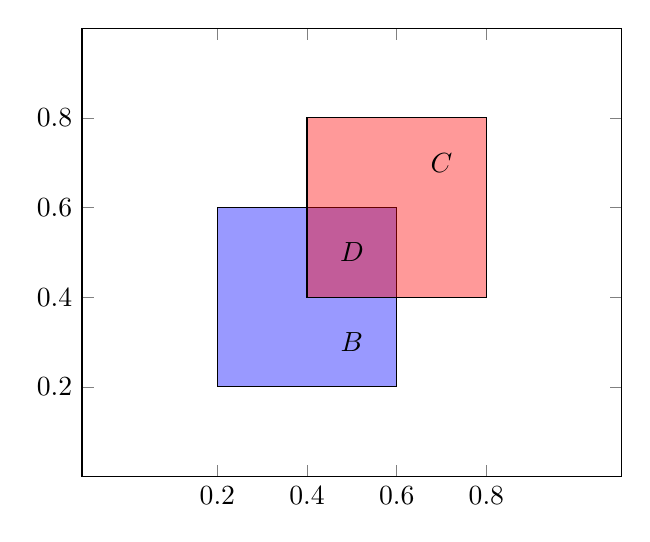
\begin{tikzpicture}
		\begin{axis}[xmin = 0, xmax = 1, ymin=0, ymax = 1, axis equal,
			xtick = {0.2, 0.4, 0.6, 0.8}, ytick = {0.2, 0.4, 0.6, 0.8},
			clip = false]
			\fill[blue, fill opacity=0.4, draw=black] (0.2, 0.2) rectangle (0.6, 0.6);
			\fill[red, fill opacity=0.4, draw=black] (0.8, 0.8) rectangle (0.4, 0.4);
			\node at (0.5, 0.3) {$B$};
			\node at (0.7, 0.7) {$C$};
			\node at (0.5, 0.5) {$D$};
		\end{axis}
	\end{tikzpicture}
\end{center}

Let $B \coloneqq A \setminus D, C \coloneqq A \setminus D, D \coloneqq [0.4, 0.6]^2$.
Then
\begin{align*}
	\mathbb P(N_{B \cup D = 4}, N_{C \cup D = 4}) &= \sum_{k=0}^4 \mathbb P(N_D = k) \underbrace{\mathbb P(N_{B \cup D} = 4, N_{C \cup D} = 4 \mid N_D = k)}_{\mathbb P(N_B = 4 - k, N_C = 4 - k)} \\
												  &= \sum_{k=0}^4 \mathbb P(N_D = k) \mathbb P(N_B = 4 - k) \mathbb P(N_C = 4 - k) \\
												  &= \sum_{k=0}^4 \Poisson(k; \lambda \size{D}) \Poisson(4 - k; \lambda \size{B})^2
												  \approx \num{0.023902}
\end{align*}
where we have used that $N_B, N_C$ are independent since $B, C$ are disjoint.

\subsection{(d)}
Improper prior $\pi(\lambda) \propto_\lambda 1/\lambda \propto_\lambda \GammaDist(0, 0)$
Likelihood: $\pi(\text{data} \mid \lambda) = \Poisson(\lambda \cdot 1^2)$.
Due to the Poisson-Gamma conjugacy: $\pi(\lambda \mid \text{data}) = \GammaDist(36, 1)$

\subsection{(g)}
We have that $Y \mid \lambda \sim \Poisson(\lambda \lvert D \rvert)$,
where $D$ is the disk of radius $0.1$ centered at $(0.5, 0.5)$,
$\lvert D \rvert = \pi 0.1^2$.
Since the posterior of $\lambda$ is known to be a Gamma distribution, using
$$ X \sim \GammaDist(\alpha, \beta) \implies cX \sim \GammaDist(\alpha, \frac\beta c) \quad \forall c>0 $$
we see that
$$ \frac{\size{D}}{\size{[0, 1]^2}} \lambda \mid \text{data} = \size{D} \lambda \mid \text{data}
\sim \GammaDist(36, \frac1{\size{D}}) $$
Due to Poisson and Gamma being conjugate distributions we get
$$ Y \mid \text{data} \sim \NegBin(36, 1 - \frac1{1 + \frac1{\size{D}}}) $$

\section{Question 2}
We have a contiuous-time, discrete state space Markov Chain with three states.
The vector for the holding times is: $q = (1/5, 1, 1/2)$.
The transition matrix for the embedded Markov chain is: 
$$ \tilde{P} = \begin{bmatrix}
0 & 0.5 & 0.5\\
0.5 & 0 & 0.5\\
0.5 & 0.5 & 0
\end{bmatrix} $$
\begin{enumerate}[label=(\alph*)]
	\item Compute the generator matrix Q and the limiting distribution.
	\item 
\end{enumerate}
\subsection{(a)}
By multiplying the expected holding times, $q$, with the probability of moving to each other state, specified by $\tilde{P}$, we get: 
$$ \hat{Q} = \begin{bmatrix}
0 & 0.1 & 0.1\\
0.5 & 0 & 0.5\\
0.25 & 0.25 & 0
\end{bmatrix}.$$
To get the generator matrix $Q$, we make sure each row sums to 0. $\implies$
$$ Q = \begin{bmatrix}
-0.2 & 0.1 & 0.1\\
0.5 & -1 & 0.5\\
0.25 & 0.25 & -0.5
\end{bmatrix}.$$
To get the limiting distributions we take the matrix exponential with a high $t$.
$$ e^{50Q} = \begin{bmatrix}
0.625 & 0.125 & 0.25\\
0.625 & 0.125 & 0.25\\
0.625 & 0.125 & 0.25
\end{bmatrix}.$$

\subsection{(b)}
\subsection{(c)}

\begin{comment}
	\appendix
	\section{Appendix, R code}
	\lstinputlisting[language=R]{ass2.R}
\end{comment}

\end{document}
